% This is samplepaper.tex, a sample chapter demonstrating the
% LLNCS macro package for Springer Computer Science proceedings;
% Version 2.20 of 2017/10/04
%
\documentclass[runningheads]{llncs}
%
\usepackage{graphicx}
\graphicspath{{images/}}
% Used for displaying a sample figure. If possible, figure files should
% be included in EPS format.
\usepackage{amsmath}
\usepackage[hyphens, spaces]{url}
% If you use the hyperref package, please uncomment the following line
% to display URLs in blue roman font according to Springer's eBook style:
\usepackage{hyperref}
\renewcommand\UrlFont{\color{blue}\rmfamily}
\usepackage[linesnumbered, ruled]{algorithm2e}
\usepackage{mathtools} % for coloneqq
\usepackage{subfig}

\begin{document}
%
\title{Building the simulator\thanks{Supported by the Engineering and Physical Sciences Research Council.}}
%
%\titlerunning{Abbreviated paper title}
% If the paper title is too long for the running head, you can set
% an abbreviated paper title here
%
\author{Thomas McSweeney\inst{1}\orcidID{0000-0001-9866-2229} }
%
\authorrunning{T. McSweeney}
% First names are abbreviated in the running head.
% If there are more than two authors, 'et al.' is used.
%
\institute{University of Manchester, Manchester, UK, M13 9PL \\
	\email{thomas.mcsweeney@postgrad.manchester.ac.uk} }
%
\maketitle              % typeset the header of the contribution
%
\begin{abstract}
Here we briefly summarize how we implemented our simple CPU-GPU scheduling simulator and attempt to explain why we made the choices we did.     

\keywords{GPU computing  \and static scheduling \and task-based programming.}
\end{abstract}


\section{Model and assumptions}
\label{sect.model_and_assumptions}


First we explicitly define our aim: to find the optimal schedule for a given DAG and target platform, where the optimal schedule is that which minimizes the {\em makespan} of the DAG, the total runtime of the application it represents. In fact, although we typically assume that all DAG weights correspond to times, they may actually represent anything else we wish to minimize, such as energy consumption, so long as this is done in a consistent manner. We do not however consider the simultaneous optimization or tradeoff between two or more different variables.    

We make the following assumptions about the processing resources and applications that we consider:
\begin{enumerate}
	\item Processing resources can only execute a single task at any one time.
	\item All tasks are atomic and cannot be divided across multiple processing resources. 
	\item All tasks can be executed on all processing resources, albeit with different processing times. 
	\item The DAG is given and, in particular, we have no input in how tasks are defined.
	\item We do not concerned with data locality before or after the scheduling of the DAG.
\end{enumerate} 
Note that the second assumption may not literally be true but is assumed to be so for the current level of scheduling. For example, it could be that a task consisting of multiple subtasks is scheduled on a single processor and then at a lower level those subtasks are allocated to the cores of the processor.

The third assumption means in particular that we do not consider constraints imposed by e.g., processor cache size. As GPUs have grown more and more widely-used for general purpose computations, the range of tasks which they are incapable of performing at all has dwindled so this is not as restrictive as it once was.

The fourth assumption can be more important than it may appear. For example, for Cholesky factorization, exactly how the matrix is tiled---i.e., the size of the tiles and thus the tasks in the DAG---is usually guided by the architecture on which the algorithm is to be executed since GPUs are much better suited to large tile sizes than CPUs. In future work we intend to consider the related problem of how to construct more amenable task graphs for a given application. 

The final assumption has two prongs. Firstly, since we make no assumptions about where data is initially located, we assume all entry tasks of the DAG---those with no predecessors---can be executed immediately by all workers and we do not consider, for example, the additional cost of moving data corresponding to an entry task to a GPU if that is where we decide it should be scheduled. Secondly, we also do not consider any additional costs incurred by any necessary final collation or synchronization step, such as moving all data in GPU memory registers to main memory. Ultimately our goal is only to minimize the time from when the first task is scheduled to when all tasks have been successfully executed.


\section{Why create our own simulator?}
\label{sect.why}

As previously stated, many modern runtime systems do not ever operate on the entire task DAG at once and thus do not permit the kind of static scheduling that we wish to consider here. Since our aim is to investigate whether static scheduling is in fact inherently unsuited to multicore CPU and GPU environments, we cannot do this by working within the confines of a runtime system that may implicitly assume this is the case. Likewise, sophisticated software exists that allows the realistic simulation of DAG scheduling and execution on arbitrary platforms. In particular, we considered the use of SimGrid \cite{simgrid} because of its comparability with StarPU and the continuing collaboration between the two development teams \cite{stanisic15,stanisic2014modeling}. (The idea being that users can create efficient application code with StarPU and simulate its execution on arbitrary target platforms with SimGrid.) 

Ultimately however we decided to create our own custom simulation environment in the belief that this would give us greater flexibility to experiment than any existing software would. The downside of course is that any results we gather will certainly be less reliable than those obtained on real systems or through more established simulation software such as SimGrid. However we have made the source code available in its entirety at the following Github repository so that interested researchers can analyze the choices we made in its implementation and repeat our experiments for themselves if they so desire:

\href{https://github.com/mcsweeney90/python-simulator}{{\tt https://github.com/mcsweeney90/python-simulator}}.

\noindent
Any feedback, comments or suggestions with regards to any aspect of our simulator software would be greatly appreciated. Once we have prototyped and refined promising approaches in this framework, we intend to evaluate their performance for real platforms in future work. 

Of course, we freely concede that there may be many other practical reasons why runtime system developers may not permit wholly static scheduling other than a belief that it is unsuitable, so we acknowledge the risk that the static heuristics we develop here may be difficult to put into practice. A good compromise solution may be something along the lines of the {\tt starpu\_replay} module in StarPU, which outputs for users the entire task dependency DAG of an application based on execution traces, as well as the {\em performance model} used for predicting the DAG weights. The scheduling and execution of this DAG can then be simulated offline, so users may evaluate the performance of any scheduling algorithms---static or otherwise---that they desire. In this case, a static schedule can even be fed back into the runtime system for use when the application is next executed, despite the fact that the runtime system typically only permits dynamic scheduling \cite[Sect.~3.18]{thibault:tel-01959127}. 

\section{Gathering data}
\label{sect.gathering_data}

To guide our development of the custom simulator we gathered some data from a single CPU-GPU node of a local computing cluster that we have access to, with four octacore Intel (Skylake) Xeon Gold 6130 CPUs running at 2.10GHz with 192GB RAM and four Nvidia V100-SXM2-16GB (Volta) GPUs, each with 16GB GPU global memory, 5120 CUDA Cores and NVLink interconnect. 

The first assumption we built into the simulator was motivated by the different manner in which we generally program CPUs and GPUs: we consider CPU cores individually but regard entire GPUs as discrete. To avoid ambiguity around whether we are referring to an entire processor or just a core, from now on we will refer to all discrete processing resources as {\em workers}. For example, we would regard our local node as comprising $4 \times 8 = 32$ CPU workers but only 4 GPU workers. In fact, we assume that the node effectively only comprises 28 CPU workers, following the convention that one of the CPU cores is dedicated to managing each GPU, as is often done in runtime systems such as StarPU \cite{augonnet2011starpu}. 

To get some idea of how we can realistically model task execution times on CPU and GPU workers, we considered the four BLAS kernels used in Cholesky factorization. In tiled numerical linear algebra algorithms for CPU and GPU, tile sizes typically range from $\approx 100-1000$, since the optimal CPU tile size is around about the former and the latter is the largest tile size which tends to be practical for a CPU (GPUs can of course handle much larger tile sizes with ease). For simplicity, we assume that all tiles are the same size, as our assumption is that we are initially agnostic as to which worker type a tile should be executed on. (Again, we intend to consider the related problem of constructing optimal task DAGs for given applications in future work.)   

The Intel {\em Math Kernel Library} (MKL) implementations of BLAS kernel routines are hand-tuned for Intel architectures and thus almost always the most efficient when available. Figure \ref{plot.skylake_timings} shows the distribution of $1000$ timings of the MKL implementations of the four BLAS kernels on a single core of a Skylake CPU. The timings shown are for the {\tt double} data type implementations (hence the {\tt D} preceding the kernel name) for matrices with randomly-generated entries; preliminary results suggest there do not appear to be any significant differences for {\tt single} data types. Here we show the data for tile sizes 128 and 1024 only but general trends for other tile sizes in the range appear to be similar.

\begin{figure}
	\centering	
	\subfloat[$nb = 128$]{\label{plot.skylake_timings_128}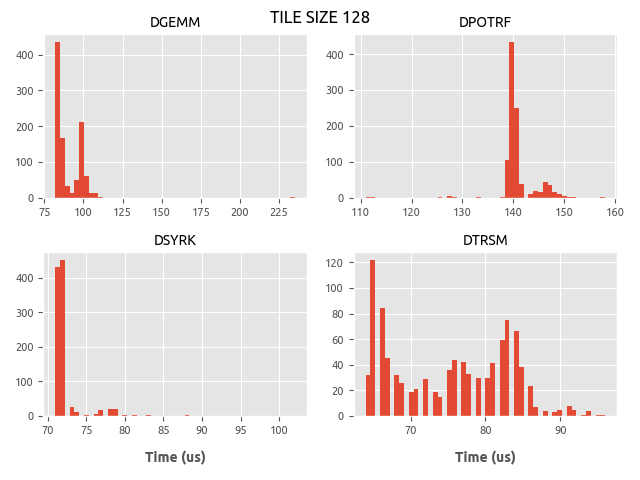
\includegraphics[scale=0.7]{skylake_cholesky_blas_tile128_histograms.png}}\\	
	\subfloat[$nb = 1024$]{\label{plot.skylake_timings_1024}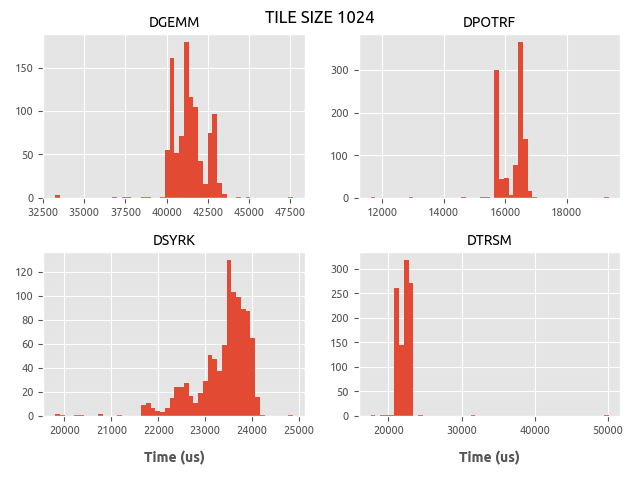
\includegraphics[scale=0.7]{skylake_cholesky_blas_tile1024_histograms.png}}
	\caption{Cholesky BLAS kernel timings on a single core of Skylake.}	
	\label{plot.skylake_timings}
\end{figure} 

Figure \ref{plot.v100_timings} shows the timing distributions when we repeat the procedure for a V100 GPU. For the {\tt DGEMM}, {\tt DSYRK} and {\tt DTRSM} kernels we use the implementations from the NVIDIA cuBLAS library, but as there is no {\tt DPOTRF} in that library we use the cuSOLVER library implementation instead for that kernel. We see that the distributions are broadly similar to the Skylake core, in that the majority are within a narrow band but there are occasional outliers that are significantly slower.
\begin{figure}
	\centering	
	\subfloat[$nb = 128$]{\label{plot.v100_timings_128}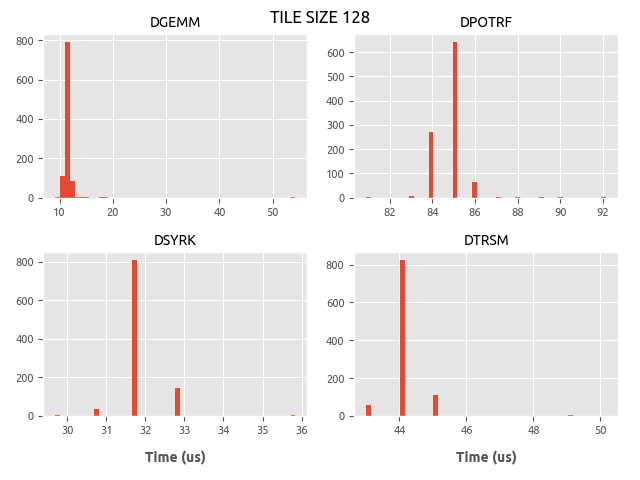
\includegraphics[scale=0.7]{V100_cholesky_blas_tile128_histograms.png}}\\	
	\subfloat[$nb = 1024$]{\label{plot.v100_timings_1024}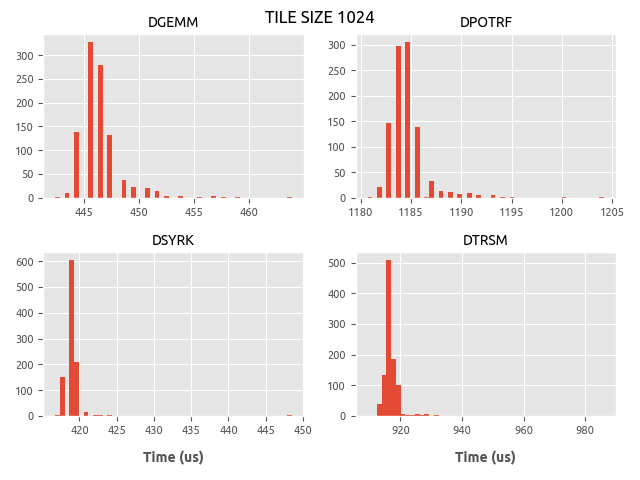
\includegraphics[scale=0.7]{V100_cholesky_blas_tile1024_histograms.png}}
	\caption{Cholesky BLAS kernel timings on V100.}	
	\label{plot.v100_timings}
\end{figure}

Given that the timing data suggest that, in general at least, CPU kernel execution times on different CPU workers will almost always likely be far more similar to one another than the corresponding GPU times (and vice versa), another assumption we built into the simulator is that all tasks have only two possible execution times---the execution time on all of the CPU workers and the execution time on all of the GPU workers. This is fairly standard in static scheduling, where the values used are acknowledged to be estimates anyway.  

When deciding whether to schedule a task on a CPU or GPU worker, what we are really interested in is the {\em acceleration ratio}, the CPU kernel execution time divided by the corresponding GPU time. Table \ref{tb.blas_routine_acc_ratios} records the mean acceleration ratios of the four Cholesky BLAS kernels for the Skylake core and V100, for different tile sizes $nb$. There are a couple of immediate takeaways. First, the acceleration ratios uniformly increase as the tile size grows larger, which we would expect given the GPU's preference for larger tile size. Second, {\tt DGEMM} consistently has the highest acceleration ratio among the kernels, and {\tt DPOTRF} the smallest. Again, we would expect this given that {\tt DGEMM}---matrix multiplication---is highly parallel, and therefore well-suited to the GPU, while {\tt DPOTRF} is the least parallelizable of the four. 
\begin{table}
	\begin{center}
	\caption{Cholesky BLAS kernel acceleration ratios (average of 1000 timings).}\label{tb.blas_routine_acc_ratios}
	\begin{tabular}{|l|l|l|l|l|}
		\hline
		{\bf Kernel}  & $nb = 128$ & $nb = 256$ & $nb = 512$ & $nb = 1024$\\
		\hline
		{\tt DGEMM} & 7.9 & 35.0 & 64.6 & 92.7 \\
		{\tt DPOTRF} & 1.7 & 1.7 & 5.0 & 13.7\\
		{\tt DSYRK} & 2.3 & 8.6 & 27.3 & 55.8\\
		{\tt DTRSM} & 1.7 & 4.2 & 12.8 & 24.2 \\
		\hline
	\end{tabular}
\end{center}
\end{table}

Ideally a good runtime system should enable the prediction of task execution times on specific workers to a fairly high degree of accuracy before runtime, which they typically attempt to do through simple statistical techniques such as linear regression on data gathered from previous executions. While our (admittedly small-scale and limited) experiments suggest that, the majority of the time at least, kernel execution times are fairly tight and therefore easy to model, the same is rarely assumed to be so for data movement times, which are notoriously difficult to predict at the node level because of shared resources such as buses and caches. 

Our own analysis of this for our local node was again based on experiments using the four Cholesky BLAS kernels. By observing the time taken between when a given worker completed execution of a task and another worker was able to begin execution of a child of that task, we came to the following conclusions:
\begin{enumerate}
	\item Data movement costs between CPU workers were negligible compared to other intra-worker communications.
	\item Timing fluctuations for moving the same amount of data across the bus were usually small. 
\end{enumerate}

Of course, the first conclusion is very much dependent on the memory architecture of the target platform. However, given that we are considering CPU workers on the same node, for almost all modern accelerated architectures it is likely that this will be true as in all other cases we typically need to move data across the bus, which can be expensive. With this in mind, in our simulator software we make the assumption that all intra-CPU communication costs are actually zero. 

The second conclusion means in particular that timing variations when passing a task from CPU to GPU, or from GPU to CPU, or from GPU to another GPU, were typically insignificant. Again, this is very much dependent on the system architecture, although we think it is reasonable to assume that they will usually be at least of similar magnitude on most modern architectures. This motivated another assumption we made in our simulation environment: there are effectively only two possible communication costs between tasks $A$ and $B$---0, when both $A$ and $B$ are scheduled on a CPU worker or if they're both scheduled on the same GPU, and some nonzero value $C$ when they are scheduled on different processor types or two distinct GPUs. Like any model, this is of course not wholly accurate, however the intention is that it will encode the important characteristics of the problem. It should also be borne in mind once again that in our static scheduling framework costs are acknowledged not to be precisely accurate but merely enough so that the resulting schedule will still be useful in practice. 

The idea behind using a runtime system to manage data movement is both to alleviate the burden on the programmer and reduce communication costs as much as possible. One way this is often done is {\em asynchronous data transfers}---i.e., beginning data movement from a task while its computation is still in progress. This means that we can often cover communication costs with computation, either entirely or in part, and in particular that effective communication times are likely to be considerably smaller than the kind of analysis done here would suggest. Although we do not explicitly consider asynchronous data transfers here, many of the results presented should still be broadly applicable since we vary the ratio of computation and communication for the DAGs that we use in our simulations. 

Throughout this report we typically present results for two different target platforms:
\begin{itemize}
	\item {\em Single GPU}, a node comprising 1 GPU worker and 7 CPU workers. 
	\item {\em Multiple GPU}, a node comprising 4 GPU workers and 28 CPUs workers. 
\end{itemize}
The latter represents the node of the local cluster referred to previously. The single GPU node corresponds to the resources that the cluster admins permit users not from a dedicated research group to access; the idea here is by considering a node of this also we can observe how the number of platform GPUs available affects scheduling decisions.

\section{Constructing realistic test DAGs}
\label{sect.test_DAGs}

In this report we simulate the scheduling of two different sets of DAGs. The first correspond to Cholesky factorization of $N \times N$ tiled matrices, where $N = 5, 10, 15, \dots, 40$. These comprise between $35$ and $11,480$ tasks. Results presented are for tile size $nb = 128$, although all were also repeated for tile size $nb = 1024$.  DAG weights are generated by sampling from real timing data that we gathered as described in the previous section.

The standard way to quantify the relative amount of communication and computation represented by a task graph is the {\em computation-to-communication ratio} (CCR), the mean computation cost of the entire DAG divided by the mean communication cost. Computing this is more complex than it may appear with our model of communication since nonzero costs are only incurred when two tasks are scheduled on different processor types, or two distinct GPUs; we compute it in the following way. First, define $w_C(t)$ to be the CPU execution time of task $t$ and $w_G(t)$ the corresponding GPU time. Then we can define  
\begin{equation}
T_{C} = \sum_t w_C(t) \quad \text{and} \quad T_{G} = \sum_t w_G(t).
\end{equation}
Let $N_C$ be the number of CPU workers, $N_G$ the number of GPU workers and $N_W = N_C + N_G$ the total number of workers. Then the mean computation time $T_{comp}$ is 
\begin{equation}
T_{comp} = \frac{N_C \cdot T_{C} + N_G \cdot T_{G} }{N_W}.
\end{equation}
Let $C(t, s)$ be the nonzero communication cost between tasks $t$ and $s$, and $H(t)$ the set of child tasks of task $t$. Then the mean communication time $T_{comm}$ is given by
\begin{equation}
T_{comm} = \frac{N_G + N_W - 1}{N_W^2} \cdot \sum_{t} \sum_{s \in H(t)} C(t, s),
\end{equation}
where the fraction on the right-hand side is the expected fraction of the time that we expect to incur a nonzero communication cost. The CCR is then calculated as $T_{comp} / T_{comm}$.

CCR values calculated in this way for Cholesky DAGs were fairly high. For example, with tile size $nb = 128$ the CCR was usually about 2 on the single GPU node and about 6 on the multiple GPU node, with minor variation depending on the total number of tasks in the DAG. (For tile size $nb = 1024$, the respective values were 32 and 117.)

As this represents only a single application, in an attempt to consider as wide a range of applications as possible we also constructed a randomized set of DAGs. Tobita and Kasahara \cite{Tobita2002} propose a set of task graphs for benchmarking scheduling algorithms and heuristics, called the Standard Task Graph set, which are freely available for download online at . This is a collection of 2700 task graphs, 180 each of a given size (i.e., the total number of tasks) from 50 to 5000, with additional single entry and exit tasks (so actually between 52 and 5002 tasks in total). The DAGs were generated via several different standard methods with the intention of capturing as wide a variety of features (degree of parallelism, edge density, etc) as possible. We use the size 1002 DAG topologies from the STG but, rather than using the costs provided, attempt to generate our own in a reasonable way. 

Following the approach in \cite{canon2018}, we generate task execution times by choosing GPU times uniformly at random from the interval $[1, 100]$ and computing CPU execution times by multiplying the GPU time by a random variable from a Gamma distribution. Based on the range of acceleration ratios we observed in our own experimentation with linear algebra kernels, this distribution was defined with both mean and standard deviation 40. The CCRs for Cholesky DAGs varied depending on the tile size and the composition of the platform, ranging from 1.8 to well over 100, and we also wished to observe the effect of very low CCR values. So for each DAG from the STG set, we generate three topologically identical copies, with communication costs randomly generated such that the CCR falls in the intervals $[0, 1]$, $[1, 5]$ or $[5, 100]$. (Hence for each CCR range there are 180 DAGs to test on.) 

\subsection{An example: tiled Cholesky factorization}
\label{subsect.cholesky}

An example of how an application can be transformed to a DAG comes from numerical linear algebra. Typically in task-based linear algebra algorithms, tasks are {\em Basic Linear Algebra Subprograms} (BLAS) kernel calls on tiles of a matrix \cite{tdb10}. The BLAS are a specification for efficient implementations of common linear algebra operations, such as matrix multiplication \cite{dongarra1988extended}. For example, Algorithm \ref{alg.tile_Cholesky} outlines how the Cholesky factorization of a (symmetric, positive definite) matrix $A$ can be computed. Note that we make use of only four BLAS kernels in total: {\tt GEMM} (matrix multiplication), {\tt POTRF} (Cholesky factorization), {\tt SYRK} (symmetric rank-$k$ update) and {\tt TRSM} (triangular solve). From this algorithm, we can easily construct the corresponding task dependency DAGs for matrices of arbitrary size by tracking the dataflow; for example, Figure \ref{plot.Cholesky_DAG} is the task DAG formed using this method for a $5 \times 5$ tile matrix $A$.

\begin{algorithm}	
	
	\SetKwInOut{Input}{Input}
	\SetKwInOut{Output}{Output}
	
	\Input{Symmetric positive definite matrix $
		A = \begin{bmatrix}
		A_{11} & A_{12}\\
		A_{12} & A_{22}
		\end{bmatrix}$.
	}	
	\Output{Lower triangular matrix $L$ such that $A = LL^T$. For efficiency, the matrix $A$ is overwritten such that $
		A = \begin{bmatrix}
		L_{11} & \\
		L_{12} & L_{22}
		\end{bmatrix}$.}
	
	
	\While{$A$ is not fully factorized}
	{
		Update $A_{11} = {\tt POTRF}(A_{11}) \coloneqq L_{11}$
		
		Compute $A_{12} = A_{12}L_{11}^{-T} \coloneqq L_{12}$ using {\tt TRSM}
		
		Compute $A_{22} = A_{22} - L_{21} L_{21}^{T} \coloneqq L_{22}$ using {\tt SYRK} and {\tt GEMM}
		
		$A = A_{22}$
	}		
	
	\caption{A practical algorithm for computing the Cholesky factorization of a matrix using BLAS kernels.}
	\label{alg.tile_Cholesky}
\end{algorithm} 

\begin{figure}
	\centering	
	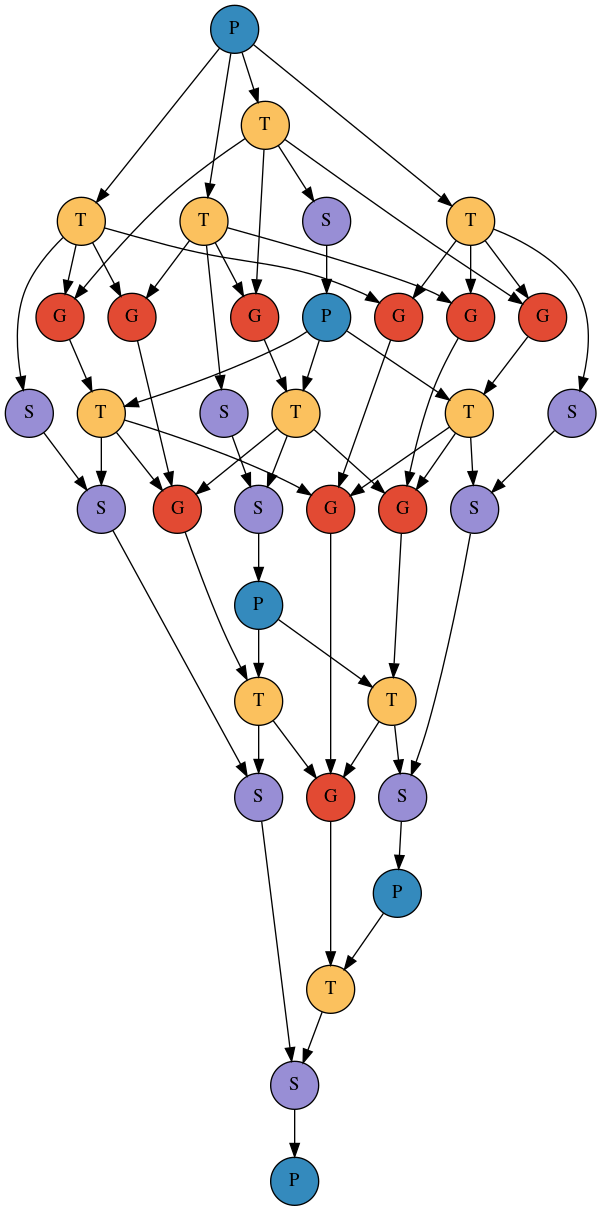
\includegraphics[width=0.5\textwidth]{Cholesky_35tasks_DAG.png}		
	\caption{Cholesky factorization of a $5 \times 5$ tiled matrix $A$. }
	\label{plot.Cholesky_DAG}	
\end{figure}  


\subsection{An example: implementing HEFT}
\label{subsect.implementing_HEFT}

Suppose we have a DAG $G$ with $v$ tasks and $e$ edges. Let $N_C$ be the number of CPU workers, $N_G$ the number of GPU workers and $N_W = N_C + N_G$ the total number of workers that comprise the target platform. Let $w_{ij}$ be the estimated time it takes to execute task $t_i$ on worker $p_j$. Then we define the {\em average execution cost} of task $t_i$ by
\begin{equation}
\label{eq.avg_weight}
\overline{w_i} = \sum_{j = 1}^{N_W} w_{ij} / N_W.
\end{equation}  

Let $d_{ij}$ be the amount of data that needs to be transferred from task $t_i$ to task $t_j$ (which will of course be zero if no dependency exists). Let $b_{mn}$ be the data transfer rate between workers $p_m$ and $p_n$ (i.e., the {\em bandwidth}). In out model, since all intra-CPU communications are assumed to be zero then we can regard the bandwidth to effectively be infinite in that case, and the only bandwidth we are actually concerned with is the interconnect bandwidth $b_{I}$, which we further assume to be constant and identical between all relevant workers---i.e., we have $b_{mn} = b_{I}$, assuming $m \neq n$ and $p_m$, $p_n$ are not both CPU workers. The communication cost from task $t_i$ scheduled on $p_m$ to task $t_j$ scheduled on $p_n$, is thus given by
\begin{align*}
c_{ij} &= 0 \quad \text{if } p_m, p_n \in CPUs \text{ or } m = n,\\
&= \frac{d_{ij}}{b_{I}} \quad \text{otherwise}.
\end{align*} 
The {\em average communication cost} of the edge from task $t_i$ to task $t_j$ is basically the expected cost given that we make no assumptions on which workers the two tasks are scheduled on, so we can compute it as
\begin{align}
\label{eq.avg_comm}
\overline{c_{ij}} = \frac{N_G + N_W - 1}{N_W^2} \cdot  \frac{d_{ij}}{b_I}.
\end{align}
Often in similar frameworks communication costs are also calculated by adding $L_m$, the {\em communication startup cost} of worker $p_m$. We do not explicitly consider such costs in this report since our  experimentation on a real platform suggested that this is usually dominated by the data transfer cost. However, the real data we use to generate many of our test DAGs implicitly incorporates this.    

For all tasks $t$, we define $P(t)$ to be the set of all its {\em parent} tasks---its immediate predecessors in the DAG---and $C(t)$ to be the set of all its {\em child} tasks---its immediate successors.

Let $EST(t_i, p_m)$ be the {\em earliest start time} at which processor $p_m$ can execute task $t_i$. If $R_{m_i}$ is the earliest time at which $p_m$ is actually free to execute task $t_i$ and $AFT(t_k)$ is the time when execution of task $t_k$ is actually completed (which is assumed to be known once it has been scheduled), then we have 
\begin{align*}
EST(t_i, p_m) = \max \bigg\{ R_{m_i}, \max_{t_k \in P(t_i)} (AFT(t_k) + c_{ki}) \bigg\}.
\end{align*}
Note that $R_{m_i}$ is not necessarily the latest finish time of all tasks scheduled on $p_m$ since we may be following an {\em insertion-based} policy that allows tasks to be scheduled on a processor between two tasks that have already scheduled on it, assuming that task dependencies are still respected. The {\em earliest finish time} $EFT(t_i, p_m)$ for task $t_i$ on processor $p_m$ is then given by 
\begin{align*}
EFT(t_i, p_m) = w_{im} + EST(t_i, p_m).
\end{align*}
Once all tasks have been scheduled, the makespan of graph $G$ can then be computed as 
\begin{align*}
M(G) &= \max_{t \in G} AFT(t) \\
&= \max_{t_e \in G} AFT(t_{exit}),
\end{align*}
where $t_{exit}$ is an {\em exit} task---i.e., one with no children. 

Schedulers targeting homogeneous platforms often use the {\em upward rank} (or {\em bottom-level}) of a task to determine priorities, defined as the length of the critical path from that task to the end, including the cost of the task itself \cite{topcuoglu2002performance}. Essentially, the upward rank is the expected time from when the task is scheduled to when the execution of the whole DAG is complete. HEFT extends the idea to heterogeneous platforms by using the {\em average} computation and communication costs across all processors. More formally, for any task $t_i$ in the DAG, we define its upward rank $rank_u(t_i)$ recursively, starting from the exit task(s), by
\begin{align}
\label{eq.upward_rank}
rank_u(t_i) = \overline{w_i} + \max_{t_j \in C(t_i)} (\overline{c_{ij}} + rank_u(t_j)).
\end{align}
Note that we can also define the {\em downward rank} (or {\em top-level}) of a task, the critical path length from its source to the task in question, excluding the cost of the task itself. There doesn't seem to be any deep theoretical justification for preferring one alternative to the other but upward ranking is suggested by the original authors and comparative studies since then have found that it is almost always the more effective choice; our own simulations likewise suggest this is the case, with the exception of when communication costs are high. 

\subsection{Computing the critical path}
\label{subsect.metrics}

Speedup is generally straightforward to compute but the SLR is more complex because of ambiguity surrounding how we define the critical path for heterogeneous platforms. The most common solution in the literature is to assume that all tasks can be executed without contention on the kind of processor that minimizes their execution time (i.e., set all task weights in the DAG to their smallest possible value) and then solve for the critical path. Edge weights/communication costs are often neglected altogether, leading to a looser lower bound on the makespan. While the SLR is clearly good to know in general, it should be emphasized that the critical path is only a lower bound and may be quite loose in practice. As it is also much more expensive to compute than the speedup, we typically prefer to use that as a comparison metric instead, especially since we typically compare two or more schedules computed by different means and thus are more interested in establishing how good they are relative to each other than how close each is to optimal. 






%
% ---- Bibliography ----
%
% BibTeX users should specify bibliography style 'splncs04'.
% References will then be sorted and formatted in the correct style.
%
 \bibliographystyle{splncs04}
 \bibliography{references}

\end{document}
